\chapter{Communication Protocol}

\begin{figure}
\centering
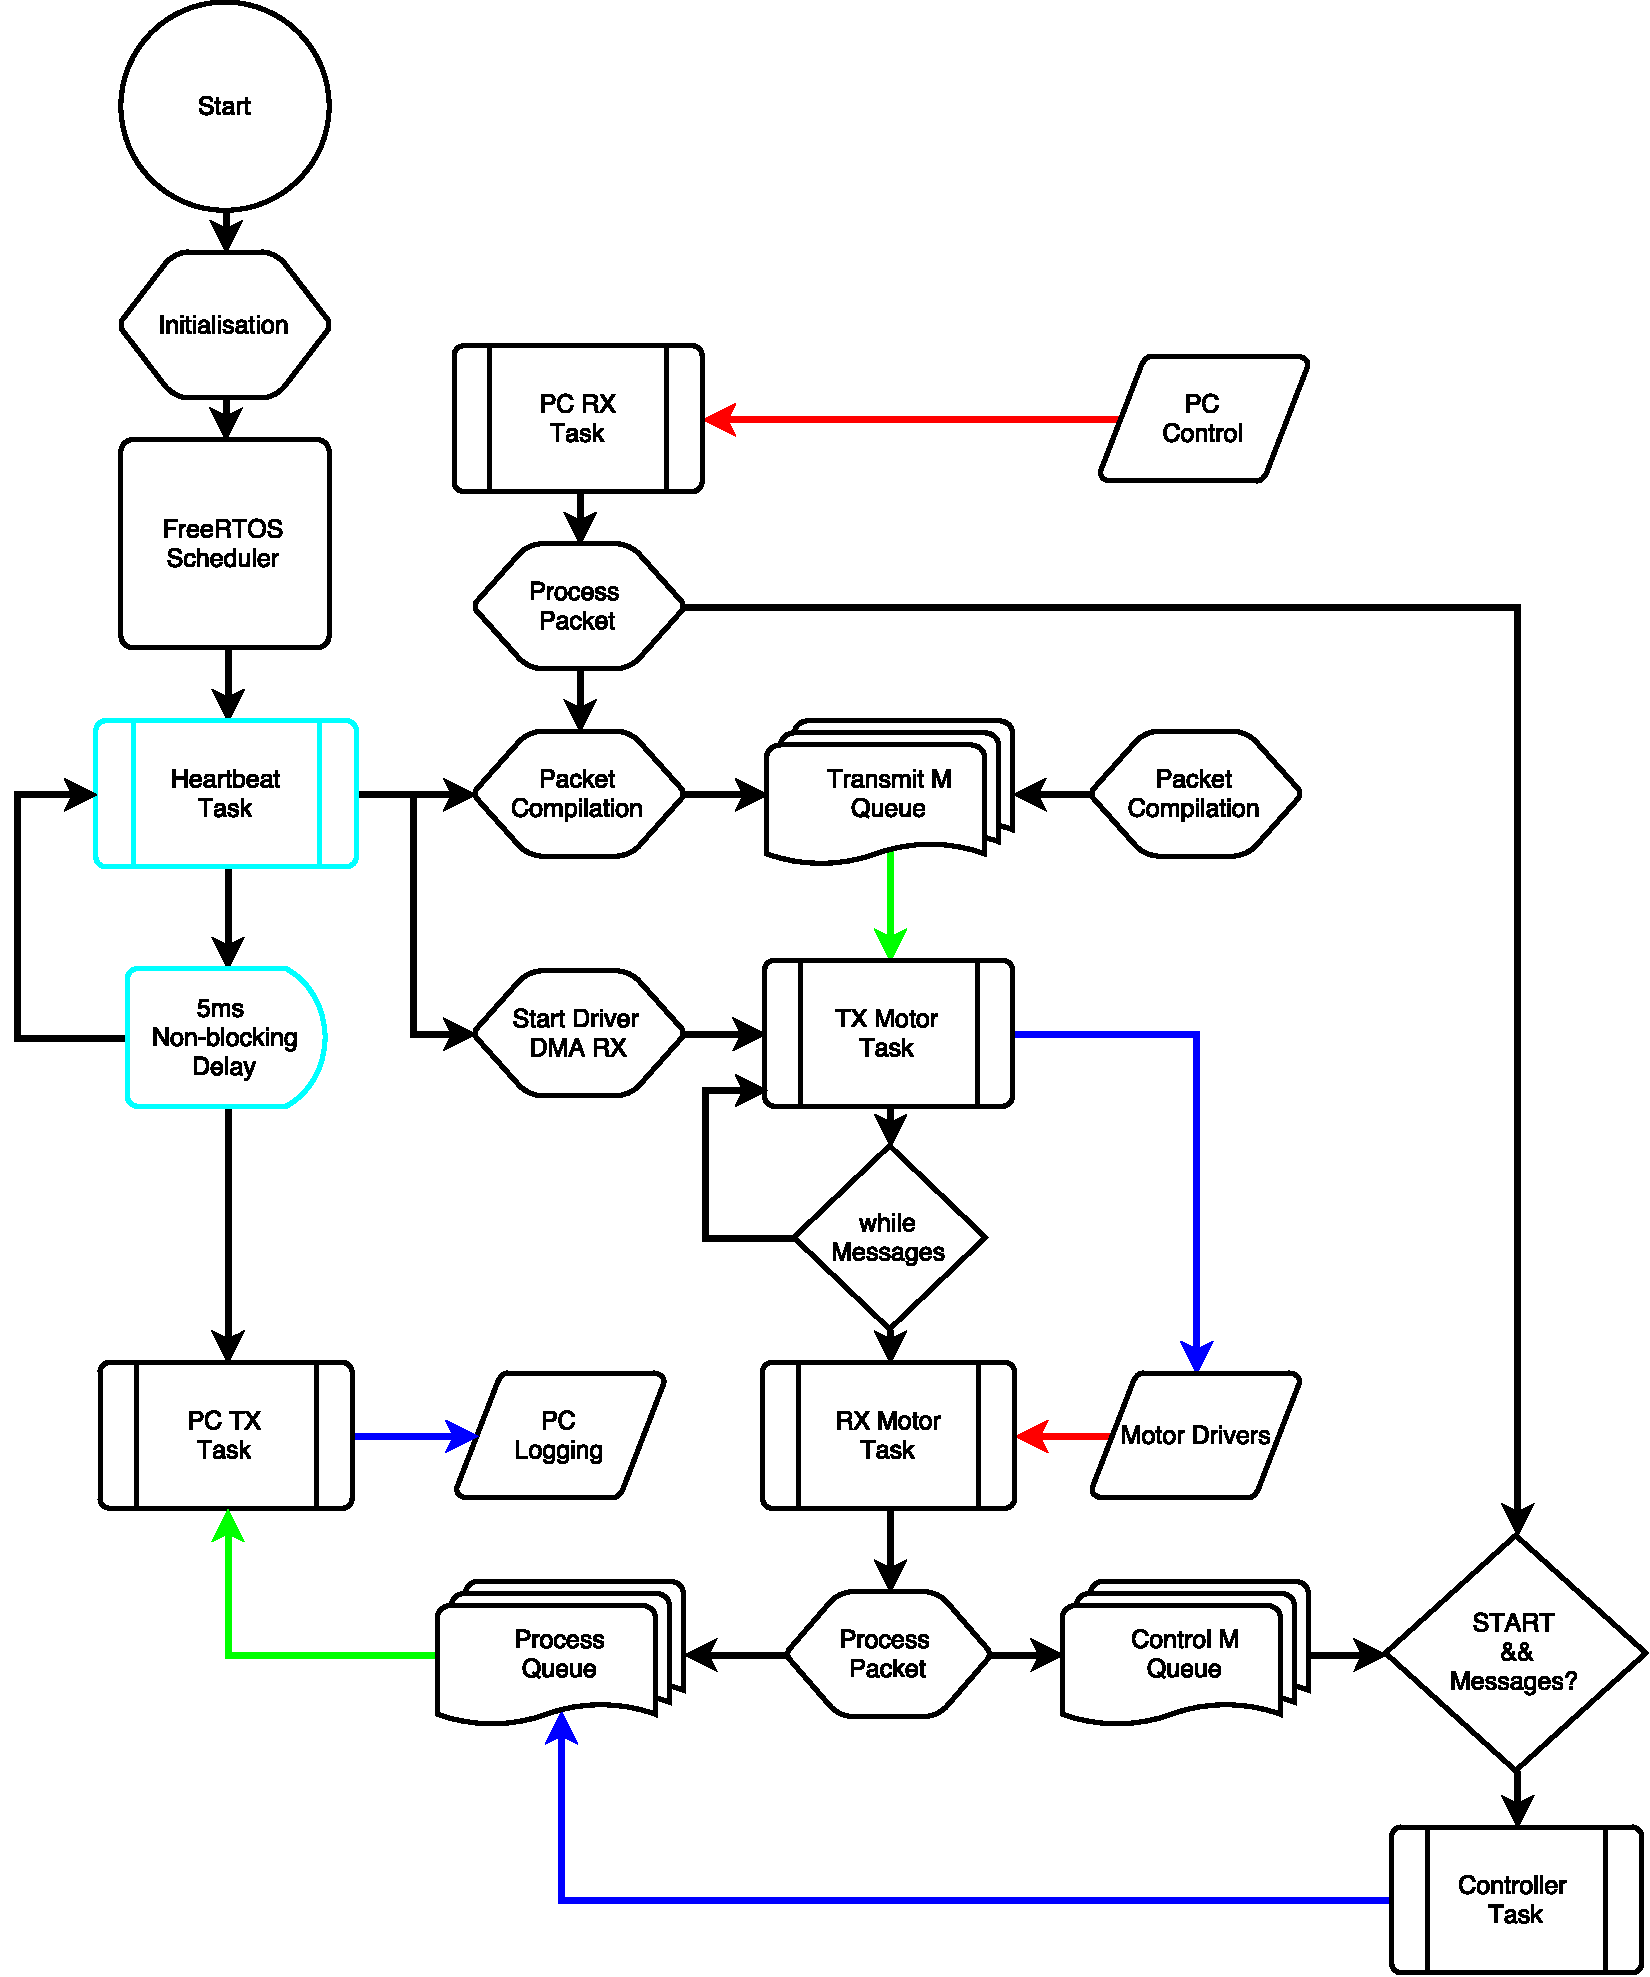
\includegraphics[width=1\textwidth]{images/comms/communication-flow-diagram.pdf} 
\caption{FreeRTOS communication protocol flow diagram.}
\label{fig:FreeRTOS communication protocol flow diagram.}
\end{figure}

A useful tool when calculating and confirming CRC values of various types: 

\url{https://www.lammertbies.nl/comm/info/crc-calculation.html}

\begin{table}[ht!]
\centering
\begin{tabular}{llllll}
\textbf{Command}       & \textbf{Index} & \textbf{Op-Code} & \textbf{TX CB} & \textbf{TX CRC1} & \textbf{RX  CB} \\
\textbf{Kill Bridge}   & 1              & 0001             & 0x06           & 0xCBB6           & 0x04            \\
\textbf{Write Enable}  & 2              & 0010             & 0x0A           & 0x3624           & 0x08            \\
\textbf{Bridge Enable} & 3              & 0100             & 0x12           & 0x1AE0           & 0x10            \\
\textbf{Set Current}   & 4              & 0011             & 0x0E           & 0xBF7B           & 0x0C            \\
\textbf{Read Current}  & 5              & 1100             & 0x31           & 0x9772           & 0x32            \\
\textbf{Read Position} & 6              & 1111             & 0x3D           & 0xD310           & 0x3E            \\
\textbf{Read Velocity} & 7              & 0101             & 0x15           & 0x5EAF           & 0x16            \\
\textbf{Set Position}  & 8              & 1010             & 0x2A           & 0x42C4           & 0x28           
\end{tabular}
\caption{Motor driver command protocol.}
\label{tab:motor-driver-protocol}
\end{table}